\subsection{Configure Sectors}
\label{sec:configure_sectors}

This dialog allows management of sectors (as in 2.5D polygons) stored in the database. \\

It is recommended if the sectors are to be used for evaluation purposes and/or if the altitude information is of use. For 2D display-only polygons it is recommended to add such information to the used map files, as described in \nameref{sec:adding_maps}. \\

Please \textbf{note} that importing at least one sector is required for using the evaluation feature later.

\begin{figure}[H]
  \center
    \hspace*{-0.5cm}
    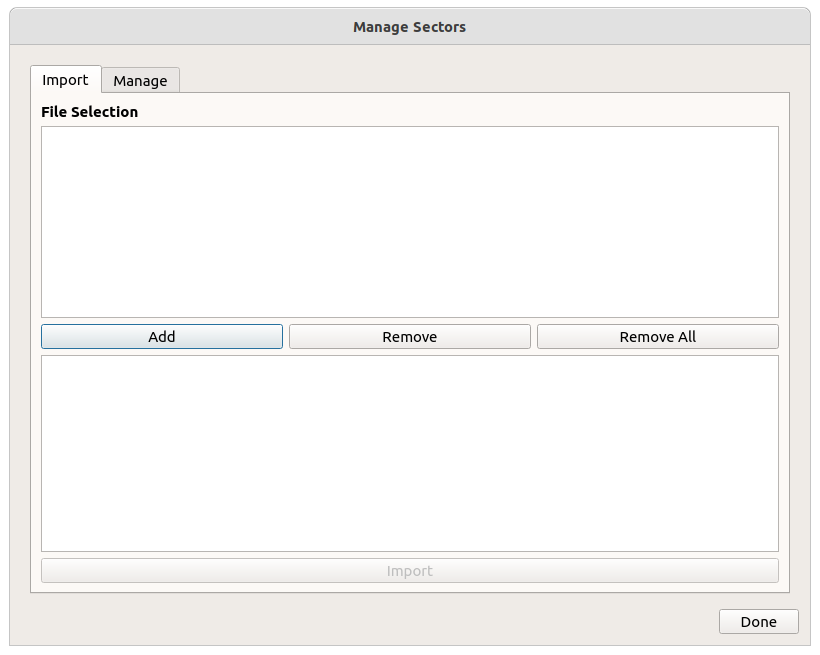
\includegraphics[width=15cm]{figures/configure_sectors.png}
  \caption{Configure Sectors}
\end{figure}

There exist 2 tabs:

\begin{itemize}
\item Import: For importing sectors from files
\item Manage: Management of imported sectors stored in the database
\end{itemize}
\ \\

\subsubsection {Import Tab}

In the 'File Selection' list, a list of available files is given. Entries can be added using the 'Add' button or removed using either the 'Remove' or 'Remove All' buttons. \\

Files are imported using the GDAL library, which can read a number of GIS files, and all encapsulated polygons or multi-polygons are written to the database with unique names. Supported common file-formats are e.g.:

\begin{itemize}
\item ESRI Shapefile
\item GML
\item KML
\end{itemize}
\ \\

Note that only polygon information is added, and all information is assumed to be stored in the WGS84 coordinate system. \\

Below a text field is given which, after selection of a file, displays the content information and/or error messages. \\\

\paragraph {Usage}

After adding an example file, the 'Import' tab looks as follows:

\begin{figure}[H]
    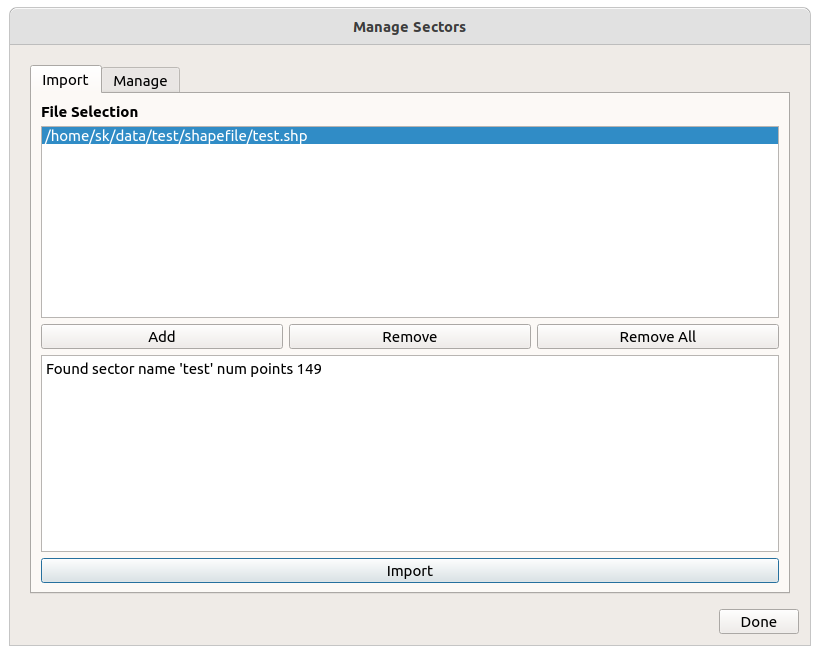
\includegraphics[width=15cm]{figures/configure_sectors_ready.png}
  \caption{Configure Sectors with example file}
\end{figure}

To import a sector, select the wanted file in the file list and press the 'Import' button, after which an import dialog is shown. \\

\begin{figure}[H]
    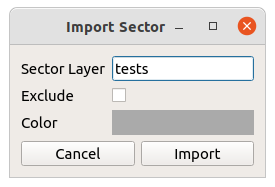
\includegraphics[width=6cm]{figures/configure_sectors_import_dialog.png}
  \caption{Configure Sectors import dialog}
\end{figure}

The following options exist:
\begin{itemize}
\item Sector Layer: Define in which sector layer the new sectors will be grouped in
\item Exclude: Define whether the imported sectors will be impored as 'Exclude' sectors
\item Color: Color to be used
\end{itemize}
\ \\

After successful import, a confirmation message is shown. \\

\paragraph {Manage Tab}

\begin{figure}[H]
    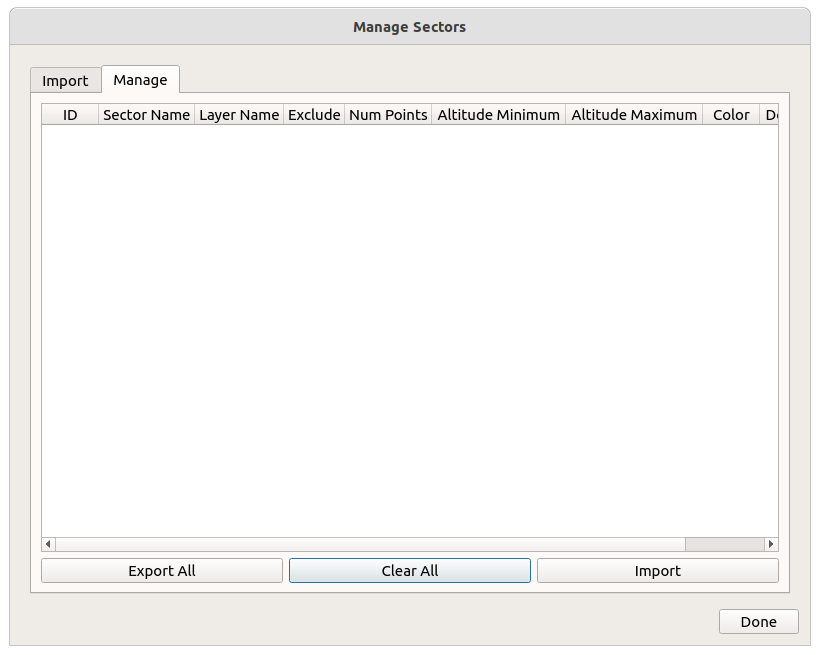
\includegraphics[width=15cm]{figures/configure_sectors_manage.png}
  \caption{Configure Sectors Manage tab}
\end{figure}

In the Manage tab, a table listing the existing sectors is given, which allows editing/deleting of the information stored in the database. \\

The following columns exist in the table:
\begin{itemize}
\item ID: Unique identifier number, read-only
\item Sector Name: Name of the sector, editable
\item Layer Name: Name of the layer the sector will be grouped in, editable
\item Exclude: Whether the sector is an 'Exclude' sector
\item Num Points: Number of points in polygon, read-only
\item Altitude Minimum: Minimum altitude in feet, editable, can be empty (gray)
\item Altitude Maximum: Maximum altitude in feet, editable, can be empty (gray)
\item Color: Color in display, editable
\item Delete: Delete button
\end{itemize}
\ \\

The 'Exclude' sector is a special case where e.g. a sector layer 'Example' has at least one normal sector 'Area', giving the 2.5d polygon in which surveillance data of interest exists. Now, to exclude target reports in a specific sector inside the bigger 'Area' sector, one or several smaller sectors can be imported (again into sector layer 'Example') and marked as 'Exclude' sectors and at best using a different color. \\

At the botton, 3 buttons exist:

\begin{itemize}
\item Export All: Saves all stored sectors as JSON file
\item Clear All: Deletes all stored sectors
\item Import: Imports a previously exported sector JSON file
\end{itemize}
\ \\

\paragraph {Usage}

After importing an sectors, the 'Manage' tab looks as follows:

\begin{figure}[H]
    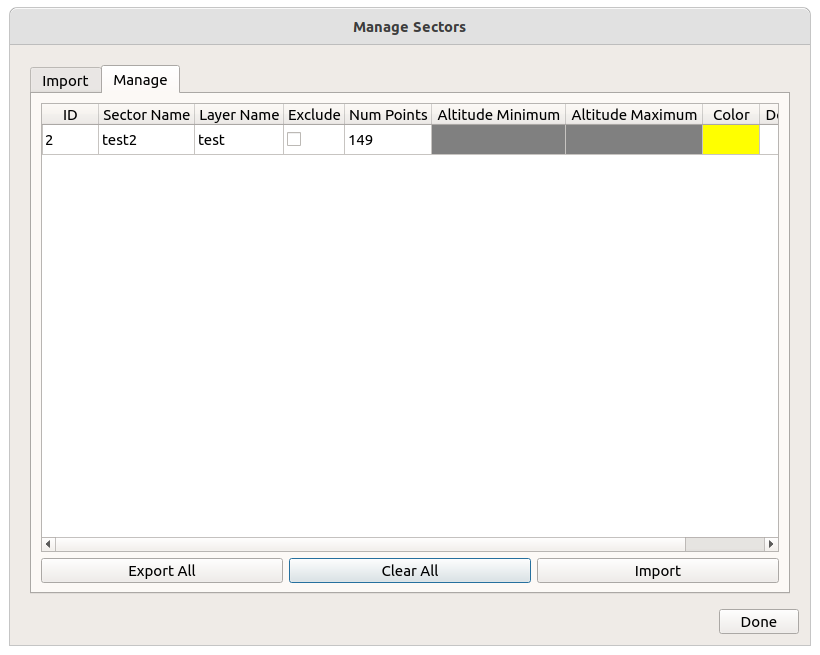
\includegraphics[width=15cm]{figures/configure_sectors_manage2.png}
  \caption{Configure Sectors with example sector}
\end{figure}

The attributes of the respective sector can be changed as wanted, by double-clicking on the text value or clicking on the color. Each change is stored immideately in the database. The result might look as follows:\\

\begin{figure}[H]
    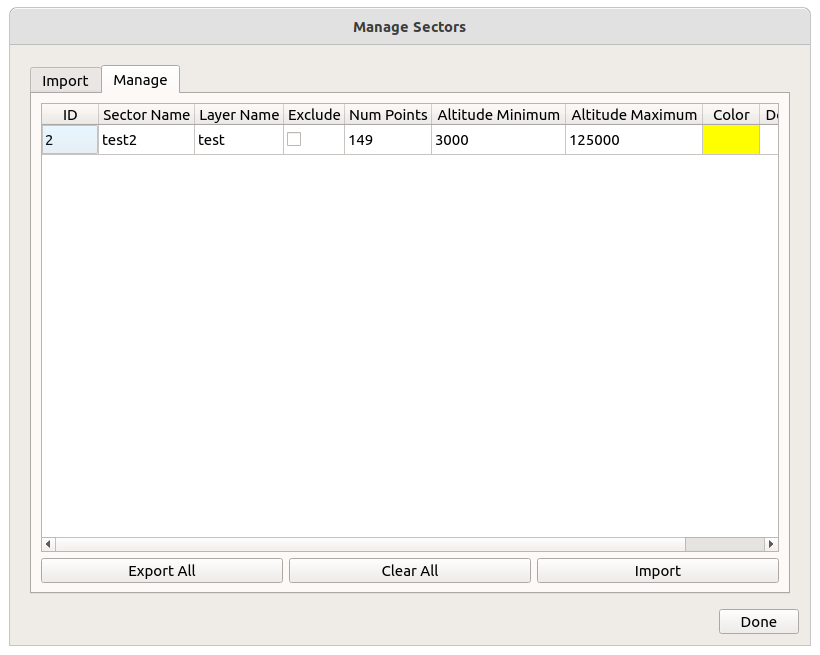
\includegraphics[width=15cm]{figures/configure_sectors_done.png}
  \caption{Configure Sectors editing result}
\end{figure}

It is recommended to export all sectors after creation, for later usage (e.g. in another database).
